\begin{figure*}
%\captionsetup{justification=centering}
\setlength\tabcolsep{2.2pt} % default value: 6pt

\begin{tabular}{c c c c c c}
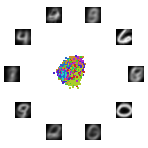
\includegraphics[height=0.16\textwidth]{experiments2_files/mnist_progression/726_run_1_colour_0_pointcloud_0.png} & 
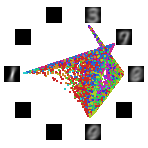
\includegraphics[height=0.16\textwidth]{experiments2_files/mnist_progression/726_run_1_colour_0_pointcloud_3.png} & 
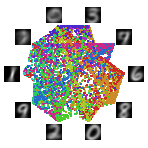
\includegraphics[height=0.16\textwidth]{experiments2_files/mnist_progression/726_run_1_colour_0_pointcloud_10.png} & 
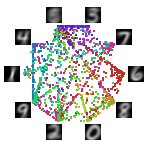
\includegraphics[height=0.16\textwidth]{experiments2_files/mnist_progression/726_run_1_colour_0_pointcloud_30.png} & 
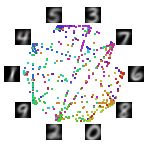
\includegraphics[height=0.16\textwidth]{experiments2_files/mnist_progression/726_run_1_colour_0_pointcloud_101.png} & 
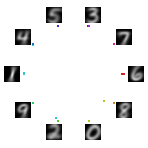
\includegraphics[height=0.16\textwidth]{experiments2_files/mnist_progression/726_run_1_colour_0_pointcloud_1000.png} 
\end{tabular}

\caption{\label{f:mnist_dots} Training with \methodnameshort on unlabelled MNIST in successive epochs from random initialisation (left). The network directly outputs cluster assignment probabilities for input images, and each is rendered as a coordinate by convex combination of 10 cluster vertices. There is no cherry-picking as the entire dataset is shown in every snapshot. Ground truth labelling (unseen by model) is given by colour. At each cluster the average image of its assignees is shown. With neither labels nor heuristics, the clusters discovered by \methodnameshort correspond perfectly to unique digits, with one-hot certain prediction (right).}
\end{figure*}